% This is "sig-alternate.tex" V2.0 May 2012
% This file should be compiled with V2.5 of "sig-alternate.cls" May 2012
%
% This example file demonstrates the use of the 'sig-alternate.cls'
% V2.5 LaTeX2e document class file. It is for those submitting
% articles to ACM Conference Proceedings WHO DO NOT WISH TO
% STRICTLY ADHERE TO THE SIGS (PUBS-BOARD-ENDORSED) STYLE.
% The 'sig-alternate.cls' file will produce a similar-looking,
% albeit, 'tighter' paper resulting in, invariably, fewer pages.
%
% ----------------------------------------------------------------------------------------------------------------
% This .tex file (and associated .cls V2.5) produces:
%       1) The Permission Statement
%       2) The Conference (location) Info information
%       3) The Copyright Line with ACM data
%       4) NO page numbers
%
% as against the acm_proc_article-sp.cls file which
% DOES NOT produce 1) thru' 3) above.
%
% Using 'sig-alternate.cls' you have control, however, from within
% the source .tex file, over both the CopyrightYear
% (defaulted to 200X) and the ACM Copyright Data
% (defaulted to X-XXXXX-XX-X/XX/XX).
% e.g.
% \CopyrightYear{2007} will cause 2007 to appear in the copyright line.
% \crdata{0-12345-67-8/90/12} will cause 0-12345-67-8/90/12 to appear in the copyright line.
%
% ---------------------------------------------------------------------------------------------------------------
% This .tex source is an example which *does* use
% the .bib file (from which the .bbl file % is produced).
% REMEMBER HOWEVER: After having produced the .bbl file,
% and prior to final submission, you *NEED* to 'insert'
% your .bbl file into your source .tex file so as to provide
% ONE 'self-contained' source file.
%
% ================= IF YOU HAVE QUESTIONS =======================
% Questions regarding the SIGS styles, SIGS policies and
% procedures, Conferences etc. should be sent to
% Adrienne Griscti (griscti@acm.org)
%
% Technical questions _only_ to
% Gerald Murray (murray@hq.acm.org)
% ===============================================================
%
% For tracking purposes - this is V2.0 - May 2012

\documentclass{acm_proc_article-me}

\begin{document}
%
% --- Author Metadata here ---
%\conferenceinfo{WOODSTOCK}{'97 El Paso, Texas USA}
%\CopyrightYear{2007} % Allows default copyright year (20XX) to be over-ridden - IF NEED BE.
%\crdata{0-12345-67-8/90/01}  % Allows default copyright data (0-89791-88-6/97/05) to be over-ridden - IF NEED BE.
% --- End of Author Metadata ---

\title{
Multimodal Person Discovery in Broadcast TV \\ 
at Mediaeval 2015
}
%
% You need the command \numberofauthors to handle the 'placement
% and alignment' of the authors beneath the title.
%
% For aesthetic reasons, we recommend 'three authors at a time'
% i.e. three 'name/affiliation blocks' be placed beneath the title.
%
% NOTE: You are NOT restricted in how many 'rows' of
% "name/affiliations" may appear. We just ask that you restrict
% the number of 'columns' to three.
%
% Because of the available 'opening page real-estate'
% we ask you to refrain from putting more than six authors
% (two rows with three columns) beneath the article title.
% More than six makes the first-page appear very cluttered indeed.
%
% Use the \alignauthor commands to handle the names
% and affiliations for an 'aesthetic maximum' of six authors.
% Add names, affiliations, addresses for
% the seventh etc. author(s) as the argument for the
% \additionalauthors command.
% These 'additional authors' will be output/set for you
% without further effort on your part as the last section in
% the body of your article BEFORE References or any Appendices.

\numberofauthors{1} 

\author{
% You can go ahead and credit any number of authors here,
% e.g. one 'row of three' or two rows (consisting of one row of three
% and a second row of one, two or three).
%
% The command \alignauthor (no curly braces needed) should
% precede each author name, affiliation/snail-mail address and
% e-mail address. Additionally, tag each line of
% affiliation/address with \affaddr, and tag the
% e-mail address with \email.
%
% 1st. author
\alignauthor
Johann Poignant, Herv\'e Bredin, Claude Barras \\
       \affaddr{LIMSI - CNRS - Rue John Von Neumann, Orsay, France.}
       \email{firstname.lastname@limsi.fr}
\\
}
% There's nothing stopping you putting the seventh, eighth, etc.
% author on the opening page (as the 'third row') but we ask,
% for aesthetic reasons that you place these 'additional authors'
% in the \additional authors block, viz.
\date{30 July 2015}
% Just remember to make sure that the TOTAL number of authors
% is the number that will appear on the first page PLUS the
% number that will appear in the \additionalauthors section.

\maketitle
\begin{abstract}
Given raw TV broadcasts, each shot must be automatically tagged with the name(s) of people who can be both seen as well as heard in the shot. The list of people is not known a priori and their names must be discovered in an unsupervised way from provided text overlay or speech transcripts. The task will be evaluated on a new French corpus (provided by INA), using standard information retrieval metrics based on a posteriori collaborative annotation of the corpus.
\end{abstract}

\section{Motivation}

TV archives maintained by national institutions such as the French INA, the Netherlands Institute for Sound \& Vision, or the BBC are rapidly growing in size. The need for applications that make these archives searchable has led researchers to devote concerted effort to developing technologies that create indexes.

Indexes that represent the location and identity of people in the archive are indispensable for searching archives. Human nature leads people to be very interested in other people. However, at the moment that content is created or broadcast, it is not always possible to predict which people will be the most important to find in the future. Someone who appeared in a broadcast, but was relatively unnoticed, might suddenly start generating a buzz and become a trending topic on social networks or search engines. For this reason, it is not possible to assume that a biometric models capable of detecting an individual, will be present at indexing time. For some people such a model may not be available in advance, simply because they are not (yet) famous. In such cases, it is also possible that archivists annotating content by hand do not even know the name of the person. The goal of this task is to address the challenge of indexing people in the archive, under real-world conditions (i.e., there is no pre-set list of people to index). \\

Until very recently, research works dealt only with speaker or face identification. We can mention the works of \textit{Canseco et al.}~\cite{CANSECO--ASRU--2005, CANSECO--INTERSPEECH--2004} as the first paper that did not use biometric models to identify speakers based on pronounced names. Following works improved this idea: \cite{ESTEVE--INTERSPEECH--2007, JOUSSE--ICCASP--2009, MAUCLAIR--Odyssey--2006, TRANTER--ICASSP--2006}. However, in all the above studies, the identification error rate is very high when automatically recognized (and noisy) pronounced names are used as source of naming information. For face identification, in \cite{HOUGHTON--IS--1999, SATOH--IEEEMM--1999, YANG--ACMMM--2004, YANG--ACMMM--2005} they use written names on screen in a title box as source of identities, but the high word error rate on overlaid names transcription greatly limited the use of this source of information.

In 2011 began the REPERE challenge~\cite{BERNARD--SLAM--2013, KAHN--CBMI--2012}. It aimed at supporting research on person recognition in multi-modal conditions. The main objective of this challenge was to answer the two questions "Who speaks when?" and "Who appears when?" using any sources of information (including pre-existing biometric models and person names extracted from text overlay and speech transcripts). To assess the technology progress, annual evaluation campaigns were organized from 2012 to 2014. In this context, the REPERE corpus~\cite{GIRAUDEL--LREC--2012}, a French video corpus with multi-modal annotation, was developed. 3 consortiums composed of multiple teams (including ourselves) participated to this challenge. Thanks to this corpus, new research contributions appeared using the multi-modal aspect (\cite{BECHET--INTERSPEECH--2014, BENDRIS--CBMI--2013, BREDIN--ODYSSEY--2014, BREDIN--INTERSPEECH--2013, BREDIN--SLAM--2013, BREDIN--IJMIR--2014, FAVRE--SLAM--2013, GAY--CBMI--2014, POIGNANT--ASLP--2015, POIGNANT--SLAM--2013, POIGNANT--INTERSPEECH--2012, POIGNANT--MTAP--2015, ROUVIER--CBMI--2014})  . 

\subsection{Goal of the task}

Given raw TV broadcasts, each shot must be automatically tagged with the name(s) of people who can be both seen as well as heard in the shot. The list of people is not known a priori and their names must be discovered in an unsupervised way from provided text overlay or speech transcripts. 

Participants are provided with a collection of TV broadcasts pre-segmented into shots, along with the output of several baseline components: speaker diarization, face detection and tracking, speech transcription, video OCR and named entity detection. 

Participants are asked to provide, for each shot, the list of names of persons speaking AND appearing at the same time. The main novelty of the task is that the list of persons is not provided a priori, and person models (neither voice nor face) may not be trained on external data. The only way to identify a person is by finding their name in the audio (e.g., using speech transcription) or visual (e.g., using optical character recognition) streams and associating them to the correct person making the task completely unsupervised (i.e., algorithms not relying on pre-existing labels or biometric models). 

For each returned shot, participants are also asked to provide the evidence justifying their assertion (e.g. a short excerpt of the test set showing the person AND its name at the same time). This should help human annotators especially for people who are not yet famous. 

\begin{figure}[htb]
 \center 
 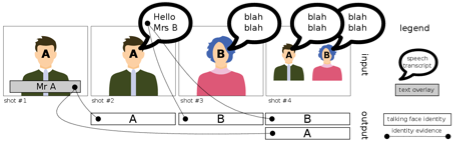
\includegraphics[width=1\linewidth]{figs/evidence.png}
 \centering
 \caption {Example of response wanted}
 \label{fig:evidence}
\end{figure}

In figure~\ref{fig:evidence}, shot \#1 is an evidence for Mr A (his name is written on screen during the shot) and shot \#3 is an evidence for Mrs B (her name is pronounced during the shot +- 5 seconds).

\section{The data set}

The original REPERE corpus set will be used as development set. It is composed of various TV shows (focusing on news, politics and people) from two French TV channels. It will be distributed by ELDA (Evaluation and Language resources Distribution Agency) freely or at distribution cost. Among those 137 hours, 50 are already manually annotated. Audio annotations are dense and provide speech transcripts and identity-labeled speech turns. Video annotations are sparse (one image every 10 seconds) and provide overlaid text transcripts and identity-labeled face segmentation. Both speech and overlaid text transcripts are tagged with named entities.

The test set is composed of French TV news provided by INA. This corpus contains 106 hours of video, corresponding to 172 editions of evening broadcast news "Le 20 heures" of French public channel "France 2", from January 1st 2007 to June 30st 2007. There is no existing annotations corresponding to our task, they were be manually created a posteriori with the help of the participant submissions.

%These videos are segmented automatically into shots. Only shots that are longer than 2 seconds should be process

\subsection{Ground truth}

Ground truth has be created a posteriori in two steps: first, by manually checking all the evidences proposed by participant. The correct evidences was used to extract mugshots that can help annotators during the second step, the manual verification of speaking faces in the shots proposed by participants.

\subsection{Metadata provided}

As the task is strongly multi-modal, we provided a large set of automatic sub-components that can help participants to process the videos (see figure \ref{fig:baseline}). The source code, in python and C++\footnote{https://github.com/MediaevalPersonDiscoveryTask/baseline}, is freely provided to participants. 

\begin{figure}[htb]
 \center 
 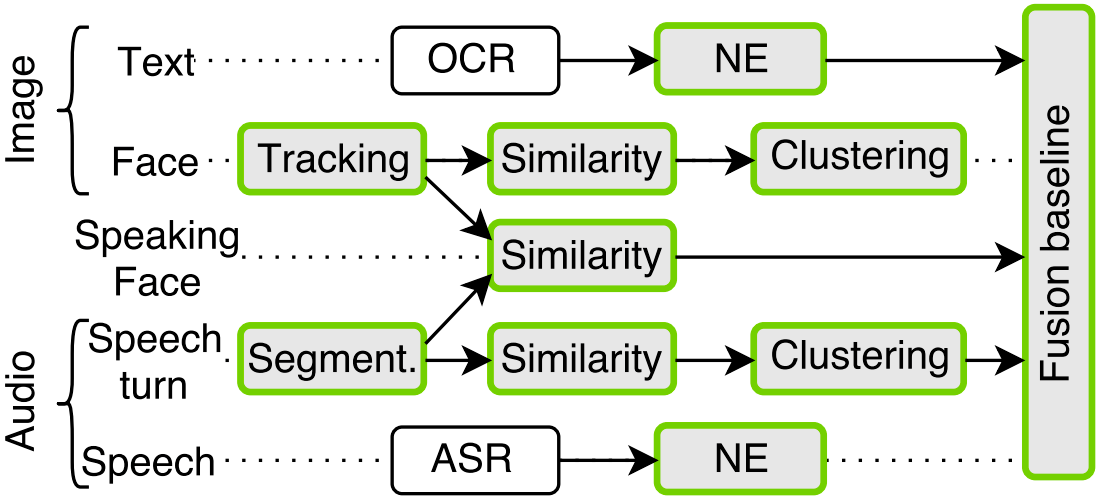
\includegraphics[width=1\linewidth]{figs/baseline.png}
 \centering
 \caption {Sub-components provided (in green)}
 \label{fig:baseline}
\end{figure}

First, we have segmented the audio stream into speech turn and detected and tracked faces on screen. Then we computed mono-modal similarities (Hog descriptors on 7 facial landmarks for faces, BIC distance for speakers) between elements (face \emph{vs} face and speech turn \emph{vs} speech turn). We also provided a similarity between speakers and co-occurring faces as in \cite{POIGNANT--MTAP--2015}. These three matrix contains probabilities and can be comparable.

Clustering was done on mono-modal matrix to try to merge all faces (respectively speech turns) of the same person (respectively speaker). 

Person names are extracted from automatic speech recognition (ASR) for pronounced names (PN) and from the optical characters recognition (OCR) (LOOV tool~\cite{POIGNANT--ICME--2012}) for written names(WN).

We also provide a fusion system baseline for participants that would only improved a sub-component. It proceed in two step, first written names are propagate onto speaker clusters \cite{POIGNANT--INTERSPEECH--2012}, then speaker identities are propagate to the speaking face with the higher similarity (according to a threshold).

\section{Evaluation procedure}

This procedure results in an Average Precision specific to the query and to the video. In order to prevent giving too much weight to predominant people or to individual video, we will first compute the Mean Average Precision over all videos where a particular person is detected, and then compute a Mean Mean Average Precision over all persons.

Average Precision will be modified slightly to take the quality of the evidence into account. Hence, instead of a binary judgment (relevant vs. not relevant), shot relevance will be computed as follows (the value of α will be discussed during the development phase):

$$ shot relevance = \alpha * shot is relevant + (1 - \alpha) * evidence is correct $$


\subsection{LeaderBoard}

As the dev set is out of domain, we propose to participants to submit their system for a second deadline one week later. Meanwhile, they have access to the MAP, compute on a secret subset of the test set, of their system performance. 

\section{Acknowledgments}

INA \\
ELDA \\
CAMOMILE \\


\newpage

% The following two commands are all you need in the
% initial runs of your .tex file to
% produce the bibliography for the citations in your paper.
\bibliographystyle{abbrv}
\bibliography{publi}  % sigproc.bib is the name of the Bibliography in this case
% You must have a proper ".bib" file
%  and remember to run:
% latex bibtex latex latex
% to resolve all references


\end{document}
